\section{Sistemas de control de versiones centralizados} 
El siguiente gran problema que se encuentra la gente es que necesitan colaborar con desarrolladores en otros sistemas. Para solventar este problema, se desarrollaron los sistemas de control de versiones centralizados (Centralized Version Control Systems o CVCSs en inglés). Estos sistemas, como CVS, Subversion, y Perforce, tienen un único servidor que contiene todos los archivos versionados, y varios clientes que descargan los archivos desde ese lugar central. Durante muchos años éste ha sido el estándar para el control de versiones

\begin{itemize}
	\begin{center}
	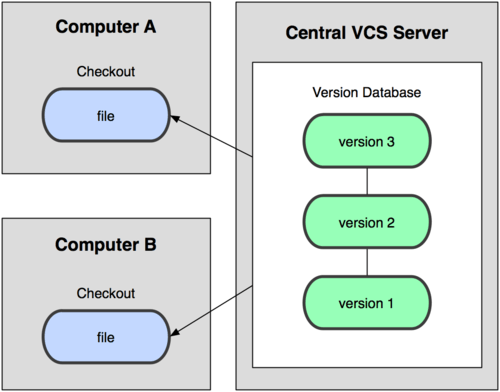
\includegraphics[width=14cm]{./Imagenes/imagen4} 
	\end{center}

	\item Esta configuración ofrece muchas ventajas, especialmente frente a VCSs locales. Por ejemplo, todo el mundo puede saber (hasta cierto punto) en qué están trabajando los otros colaboradores del proyecto. Los administradores tienen control detallado de qué puede hacer cada uno; y es mucho más fácil administrar un CVCS que tener que lidiar con bases de datos locales en cada cliente.



\end{itemize} 